\documentclass[10pt,landscape]{article}
\usepackage{multicol}
\usepackage{calc}
\usepackage{ifthen}
\usepackage{amsmath}
\usepackage{tikz}
\usepackage[landscape]{geometry}
\usepackage{hyperref}
\usepackage{caption}
\captionsetup{
   font=small,
   labelfont=bf,
   tableposition=top
}
\usetikzlibrary{decorations.markings}
\tikzset{
    set arrow inside/.code={\pgfqkeys{/tikz/arrow inside}{#1}},
    set arrow inside={end/.initial=>, opt/.initial=},
    /pgf/decoration/Mark/.style={
        mark/.expanded=at position #1 with
        {
            \noexpand\arrow[\pgfkeysvalueof{/tikz/arrow inside/opt}]{\pgfkeysvalueof{/tikz/arrow inside/end}}
        }
    },
    arrow inside/.style 2 args={
        set arrow inside={#1},
        postaction={
            decorate,decoration={
                markings,Mark/.list={#2}
            }
        }
    },
}


% To make this come out properly in landscape mode, do one of the following
% 1.
%  pdflatex latexsheet.tex
%
% 2.
%  latex latexsheet.tex
%  dvips -P pdf  -t landscape latexsheet.dvi
%  ps2pdf latexsheet.ps


% If you're reading this, be prepared for confusion.  Making this was
% a learning experience for me, and it shows.  Much of the placement
% was hacked in; if you make it better, let me know...


% 2008-04
% Changed page margin code to use the geometry package. Also added code for
% conditional page margins, depending on paper size. Thanks to Uwe Ziegenhagen
% for the suggestions.

% 2006-08
% Made changes based on suggestions from Gene Cooperman. <gene at ccs.neu.edu>


% To Do:
% \listoffigures \listoftables
% \setcounter{secnumdepth}{0}


% This sets page margins to .5 inch if using letter paper, and to 1cm
% if using A4 paper. (This probably isn't strictly necessary.)
% If using another size paper, use default 1cm margins.
\ifthenelse{\lengthtest { \paperwidth = 11in}}
	{ \geometry{top=.5in,left=.5in,right=.5in,bottom=.5in} }
	{\ifthenelse{ \lengthtest{ \paperwidth = 297mm}}
		{\geometry{top=1cm,left=1cm,right=1cm,bottom=1cm} }
		{\geometry{top=1cm,left=1cm,right=1cm,bottom=1cm} }
	}

% Turn off header and footer
\pagestyle{empty}
 

% Redefine section commands to use less space
\makeatletter
\renewcommand{\section}{\@startsection{section}{1}{0mm}%
                                {-1ex plus -.5ex minus -.2ex}%
                                {0.5ex plus .2ex}%x
                                {\normalfont\large\bfseries}}
\renewcommand{\subsection}{\@startsection{subsection}{2}{0mm}%
                                {-1explus -.5ex minus -.2ex}%
                                {0.5ex plus .2ex}%
                                {\normalfont\normalsize\bfseries}}
\renewcommand{\subsubsection}{\@startsection{subsubsection}{3}{0mm}%
                                {-1ex plus -.5ex minus -.2ex}%
                                {1ex plus .2ex}%
                                {\normalfont\small\bfseries}}
\makeatother

% Define BibTeX command
\def\BibTeX{{\rm B\kern-.05em{\sc i\kern-.025em b}\kern-.08em
    T\kern-.1667em\lower.7ex\hbox{E}\kern-.125emX}}

% Don't print section numbers
\setcounter{secnumdepth}{0}


\setlength{\parindent}{0pt}
\setlength{\parskip}{0pt plus 0.5ex}


% -----------------------------------------------------------------------

\begin{document}

\raggedright
\footnotesize
\begin{multicols}{3}


% multicol parameters
% These lengths are set only within the two main columns
%\setlength{\columnseprule}{0.25pt}
\setlength{\premulticols}{1pt}
\setlength{\postmulticols}{1pt}
\setlength{\multicolsep}{1pt}
\setlength{\columnsep}{2pt}

\begin{center}
     \Large{Hamiltonian Mechanics Cheat Sheet} \\
\end{center}

\section{Lagrangian Mechanics}
The lagrangian of a system is a function of the coordinates $\vec{q}(t)$, the velocities $\dot{\vec q}(t)$, and time.
\begin{equation}
	L = T-V 
\end{equation}

The action of a system is the time integral of the lagrangian:
\begin{equation}
	S = \int L(\vec{ q}(t), \vec {\dot q}(t), t) dt
\end{equation}

By varying the action, and finding a stable point, we get the Euler-Lagrange equations:
\begin{equation}
	\delta S = 0 = \int \left(\frac{\partial L}{\partial \vec{q}}\delta \vec{q} + \frac{\partial L}{\partial \dot{\vec q}} \delta \dot{\vec q}\right)dt = \int \left(\frac{\partial L}{\partial \vec{q}}-\frac{d}{dt} \frac{\partial L}{\partial \dot{\vec q}} \right)\delta \vec{q} dt
\end{equation}
And we get the Euler-Lagrange equations:
\begin{equation}
	\frac{\partial L}{\partial \vec{q}}=\frac{d}{dt}\frac{\partial L}{\partial \dot{\vec q}}
\end{equation}

The Euler-Lagrange equations are invariant under a change of the Lagrangian by a total time derivative:
\begin{equation}
	L \rightarrow L' = L + \frac{dF}{dt}
\end{equation}
By considering a point transformation to new coordinates $Q, \dot Q$: $Q(q, t), \dot Q(q, \dot q, t) $:
\begin{equation}
	\frac{\partial \dot q}{\partial \dot Q} = \frac{\partial q}{\partial Q}
\end{equation}
Cancellation of dots.
\section{Generalised Momenta}
The Legendre transform conjugate to the velocities $\dot{\vec q}$ are the generalised momenta $\vec{p}$:
\begin{equation}
	\frac{\partial L}{\partial \dot{\vec q}} = \vec {p}
\end{equation}
If the Lagrangian is independent of a coordinate $q$, then this is called a cyclic coordinate, and the generalised momentum is conserved:
\begin{equation}
	\frac{\partial L}{\partial q} = \frac{d}{dt}\frac{\partial L}{\partial \dot q} = \dot p = 0
\end{equation}
\section{Noether's Theorem}
If the Euler-Lagrange equations are invariant under some infinitesimal coordinate transform $\vec {q} \rightarrow \vec {q} + \epsilon \vec {w}(s_1, \mathellipsis, s_n, \vec{q}, t)$, then this transform changes the Lagrangian by a total time derivative. We can taylor expand in the infinitesimal $\epsilon$ to give:
\begin{equation}
	L - \epsilon \frac{dG}{dt} = L + \epsilon\left(\frac{\partial L}{\partial \vec{q}}\cdot\vec{w} + \frac{\partial L}{\partial \dot{\vec q}}\cdot\dot{\vec w}\right) = L + \epsilon\frac{d}{dt}\left(\frac{\partial L}{\partial \dot{\vec q}}\cdot\vec{w}\right)
\end{equation}
Which implies:
\begin{equation}
	I = G + \frac{\partial L}{\partial \dot{\vec q}}\cdot \vec{w} = \mathrm{constant}
\end{equation}
\section{The Hamiltonian}
The Hamiltonian is the Legendre transform of the Lagrangian with respect to the velocity.
\begin{equation}
	H(\vec{q}, \vec{p}, t) = \frac{\partial L}{\partial \dot{\vec q}}\cdot \dot{\vec q} - L
\end{equation}

We can get Hamilton's equations by considering the differential of H:
\begin{equation}
	dH = \frac{\partial H}{\partial \vec{q}}\cdot d\vec{q} + \frac{\partial H}{\partial \vec{p}}\cdot d\vec{p} + \frac{\partial H}{\partial t}
\end{equation}
\begin{equation}
	dH = \dot{\vec q} \cdot d\vec{p} - \dot{\vec p} \cdot d\vec{q} - \frac{\partial L}{\partial t}
\end{equation}
Equating the coefficients of the differentials, we get Hamilton's equations of motion:
\begin{equation}
	\vec v =
	\frac{d}{dt}
	\begin{pmatrix}
		\vec{q} \\
		\vec{p}
		\end{pmatrix} = 
		\begin{pmatrix}
			\nabla_{\vec{p}}H \\ 
			-\nabla_{\vec{q}}H
		\end{pmatrix}\mathrm{\ \ \ and\ \ \ } \frac{\partial H}{\partial t} = -\frac{\partial L}{\partial t}
\end{equation}

Where $\vec v$ is the phase space velocity. If the Hamiltonian is time-independent, then the motion in phase space lies along paths of constant energy:
\begin{equation}
	\vec {v}\cdot \nabla H = \nabla_{\vec{p}}H\cdot\nabla_{\vec{q}} H - \nabla_{\vec{q}}H\cdot\nabla_{\vec{p}} H = 0
\end{equation}
\section{Liouville's Theorem}

The ``fluid'' system is incompressible in phase space, and if the Hamiltonian is independent of time then the phase space fluid is constant.

Incompressibility is shown by:
\begin{equation}
	\nabla \cdot\vec{v} = \nabla_{\vec{q}}\cdot\nabla_{\vec{p}}H - \nabla_{\vec{p}}\cdot\nabla_{\vec{q}} H = 0
\end{equation}
The density $\rho$ obeys the equation:
\begin{equation}
	\frac{d\rho}{dt} = \frac{\partial \rho}{\partial t} + \nabla \cdot (\rho \vec{v}) = 0
\end{equation}
The virial theorem tells us that when averaged over time:
\begin{equation}
	\overline{\vec{p}\cdot\frac{\partial H}{\partial \vec{p}}} = \overline{\vec{q}\cdot \frac{\partial H}{\partial \vec{q}}}
\end{equation}
\section{Qualitative Dynamics}
Have systems described by a velocity $\vec {\dot r}$. These systems have fixed points at $\dot{\vec r}=\vec {0}$, which we call $\vec{r^*}$.

We can expand linearly around these fixed points to find the behaviour of the system:
\begin{equation}
\dot r^i(\vec{r^*}+\delta\vec{r}) \approx \dot r^i(\vec{r^*}) + \left.\frac{\partial \dot r^i}{\partial x^j}\right|_{\vec{r^*}} \delta r^j = A^i_j \delta r^j 
\end{equation}
Where $x^i$ are the coordinates, and the matrix $A^i_j$ is the jacobian of the velocity vector.

We can then look for solutions of $\delta \dot{\vec r}(t)=\mathbf{A}\delta\vec{r}$:
\begin{equation}
	\lambda we^{\lambda t} = \mathbf{A}\vec{w}e^{\vec{A}t}
\end{equation}
And we have an eigenvalue equation:
\begin{equation}
	\det{(\mathbf{A}-\lambda\mathbf{I})} = 0
\end{equation}
And can work out the eigenvectors:
\begin{equation}
	(\mathbf{A}-\lambda_i\mathbf{I})\vec{w}_i = 0
\end{equation}
\subsection{Eigenvalue Behaviours}
The behaviour of 2D systems for a range of eigenvalues is illstrated next.

For real and distinct eigenvalues, $\lambda_1\neq\lambda_2\neq0$, the system has the behaviours:
\begin{center}
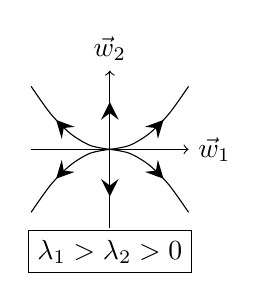
\begin{tikzpicture}
    \draw[->] (-1,0) -- (1,0) node[right] {$\vec{w}_1$};
     \draw[->] (0,-1) -- (0,1) node[above] {$\vec{w}_2$};
	%\draw[smooth, samples=100, domain=0:1] plot({\x*cos(360*\x)}, {\x*sin(360*\x)});
      \draw[smooth, samples=5, domain=0:1] plot({\x)}, {0.8*\x*\x)}) [arrow inside={end=stealth,opt={scale=2}}{0.6}];
      \draw[smooth, samples=5, domain=0:1] plot({-\x)}, {0.8*\x*\x)}) [arrow inside={end=stealth,opt={scale=2}}{0.6}];
      \draw[smooth, samples=5, domain=0:1] plot({\x)}, {-0.8*\x*\x)}) [arrow inside={end=stealth,opt={scale=2}}{0.6}];
      \draw[smooth, samples=5, domain=0:1] plot({-\x)}, {-0.8*\x*\x)}) [arrow inside={end=stealth,opt={scale=2}}{0.6}];
      \draw[smooth, samples=5, domain=0:1] plot(0, \x) [arrow inside={end=stealth,opt={scale=2}}{0.6}];
      \draw[smooth, samples=5, domain=0:1] plot(0, -\x) [arrow inside={end=stealth,opt={scale=2}}{0.6}];
	\node[draw] at (0, -1.3) {$\lambda_1>\lambda_2>0$};
\end{tikzpicture}
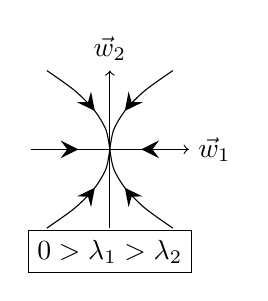
\begin{tikzpicture}
    \draw[->] (-1,0) -- (1,0) node[right] {$\vec{w}_1$};
     \draw[->] (0,-1) -- (0,1) node[above] {$\vec{w}_2$};
	%\draw[smooth, samples=100, domain=0:1] plot({\x*cos(360*\x)}, {\x*sin(360*\x)});
     \draw[smooth, samples=5, domain=1:0] plot({0.8*\x*\x}, {\x}) [arrow inside={end=stealth,opt={scale=2}}{0.6}];
      \draw[smooth, samples=5, domain=1:0] plot({0.8*\x*\x}, {-\x}) [arrow inside={end=stealth,opt={scale=2}}{0.6}];
      \draw[smooth, samples=5, domain=1:0] plot({-0.8*\x*\x}, {\x}) [arrow inside={end=stealth,opt={scale=2}}{0.6}];
      \draw[smooth, samples=5, domain=1:0] plot({-0.8*\x*\x}, {-\x}) [arrow inside={end=stealth,opt={scale=2}}{0.6}];
      \draw[smooth, samples=5, domain=1:0] plot(\x, 0) [arrow inside={end=stealth,opt={scale=2}}{0.6}];
      \draw[smooth, samples=5, domain=1:0] plot(-\x, 0) [arrow inside={end=stealth,opt={scale=2}}{0.6}];
	\node[draw] at (0, -1.3) {$0>\lambda_1>\lambda_2$};
\end{tikzpicture}
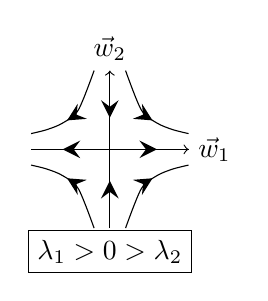
\begin{tikzpicture}
    \draw[->] (-1,0) -- (1,0) node[right] {$\vec{w}_1$};
     \draw[->] (0,-1) -- (0,1) node[above] {$\vec{w}_2$};
	%\draw[smooth, samples=100, domain=0:1] plot({\x*cos(360*\x)}, {\x*sin(360*\x)});
     \draw[smooth, samples=5, domain=0.2:1] plot({\x)}, {1/(5*\x)}) [arrow inside={end=stealth,opt={scale=2}}{0.6}];
     \draw[smooth, samples=5, domain=0.2:1] plot({-\x)}, {1/(5*\x)}) [arrow inside={end=stealth,opt={scale=2}}{0.6}];
     \draw[smooth, samples=5, domain=0.2:1] plot({\x)}, {-1/(5*\x)}) [arrow inside={end=stealth,opt={scale=2}}{0.6}];
     \draw[smooth, samples=5, domain=0.2:1] plot({-\x)}, {-1/(5*\x)}) [arrow inside={end=stealth,opt={scale=2}}{0.6}];
      \draw[smooth, samples=5, domain=0:1] plot(\x, 0) [arrow inside={end=stealth,opt={scale=2}}{0.6}];
      \draw[smooth, samples=5, domain=0:1] plot(-\x, 0) [arrow inside={end=stealth,opt={scale=2}}{0.6}];
      \draw[smooth, samples=5, domain=1:0] plot(0, \x) [arrow inside={end=stealth,opt={scale=2}}{0.6}];
      \draw[smooth, samples=5, domain=1:0] plot(0, -\x) [arrow inside={end=stealth,opt={scale=2}}{0.6}];
	\node[draw] at (0, -1.3) {$\lambda_1>0>\lambda_2$};
\end{tikzpicture}
\end{center}
An unstable repeller, a stable attractor and an unstable saddle point.

For real degenerate eigenvalues, $\lambda_1=\lambda_2\neq0$:
\begin{center}
	\begin{tikzpicture}
    \draw[->] (-1,0) -- (1,0) node[right] {$\vec{w}_1$};
     \draw[->] (0,-1) -- (0,1) node[above] {$\vec{w}_2$};
	%\draw[smooth, samples=100, domain=0:1] plot({\x*cos(360*\x)}, {\x*sin(360*\x)});
     \draw[smooth, samples=2, domain=0:1] plot({\x}, {\x}) [arrow inside={end=stealth,opt={scale=2}}{0.6}];
     \draw[smooth, samples=2, domain=0:1] plot({\x}, {0}) [arrow inside={end=stealth,opt={scale=2}}{0.6}];
     \draw[smooth, samples=2, domain=0:1] plot({\x}, -{\x}) [arrow inside={end=stealth,opt={scale=2}}{0.6}];
     \draw[smooth, samples=2, domain=0:1] plot({0}, {\x}) [arrow inside={end=stealth,opt={scale=2}}{0.6}];
     \draw[smooth, samples=2, domain=0:1] plot({0}, {-\x}) [arrow inside={end=stealth,opt={scale=2}}{0.6}];
     \draw[smooth, samples=2, domain=0:1] plot({-\x}, {\x}) [arrow inside={end=stealth,opt={scale=2}}{0.6}];
     \draw[smooth, samples=2, domain=0:1] plot({-\x}, {0}) [arrow inside={end=stealth,opt={scale=2}}{0.6}];
     \draw[smooth, samples=2, domain=0:1] plot({-\x}, -{\x}) [arrow inside={end=stealth,opt={scale=2}}{0.6}];
	\node[draw] at (0, -1.3) {$\lambda_1=\lambda_2>0$};
	\end{tikzpicture}
	\begin{tikzpicture}
    \draw[->] (-1,0) -- (1,0) node[right] {$\vec{w}_1$};
     \draw[->] (0,-1) -- (0,1) node[above] {$\vec{w}_2$};
	%\draw[smooth, samples=100, domain=0:1] plot({\x*cos(360*\x)}, {\x*sin(360*\x)});
     \draw[smooth, samples=2, domain=1:0] plot({\x}, {\x}) [arrow inside={end=stealth,opt={scale=2}}{0.6}];
     \draw[smooth, samples=2, domain=1:0] plot({\x}, {0}) [arrow inside={end=stealth,opt={scale=2}}{0.6}];
     \draw[smooth, samples=2, domain=1:0] plot({\x}, -{\x}) [arrow inside={end=stealth,opt={scale=2}}{0.6}];
     \draw[smooth, samples=2, domain=1:0] plot({0}, {\x}) [arrow inside={end=stealth,opt={scale=2}}{0.6}];
     \draw[smooth, samples=2, domain=1:0] plot({0}, {-\x}) [arrow inside={end=stealth,opt={scale=2}}{0.6}];
     \draw[smooth, samples=2, domain=1:0] plot({-\x}, {\x}) [arrow inside={end=stealth,opt={scale=2}}{0.6}];
     \draw[smooth, samples=2, domain=1:0] plot({-\x}, {0}) [arrow inside={end=stealth,opt={scale=2}}{0.6}];
     \draw[smooth, samples=2, domain=1:0] plot({-\x}, -{\x}) [arrow inside={end=stealth,opt={scale=2}}{0.6}];
	\node[draw] at (0, -1.3) {$0>\lambda_1=\lambda_2$};
	\end{tikzpicture}
\end{center}
An unstable repeller and a fixed attractor.

For $\mathbf{A}=\begin{pmatrix}\alpha & -\omega \\ \omega & \alpha\end{pmatrix}$, we have complex eigenvalues $\lambda_{\pm}=\alpha\pm i\omega$, which cause rotations.
It is easier to think polar coordinates in this case, with $\delta \dot r = \alpha \delta r$ and $\dot \theta = \omega$.
There are 3 types of fixed point in this case:
\begin{center}
	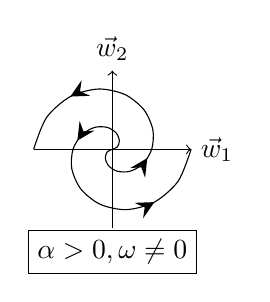
\begin{tikzpicture}
    \draw[->] (-1,0) -- (1,0) node[right] {$\vec{w}_1$};
     \draw[->] (0,-1) -- (0,1) node[above] {$\vec{w}_2$};
	\draw[smooth, samples=15, domain=0:1] plot({\x*cos(360*\x)}, {\x*sin(360*\x)}) [arrow inside={end=stealth,opt={scale=2}}{0.25, 0.75}];
	\draw[smooth, samples=15, domain=0:1] plot({-\x*cos(360*\x)}, {-\x*sin(360*\x)}) [arrow inside={end=stealth,opt={scale=2}}{0.25, 0.75}];
     \node[draw] at (0, -1.3) {$\alpha>0, \omega\neq0$};
	\end{tikzpicture}
	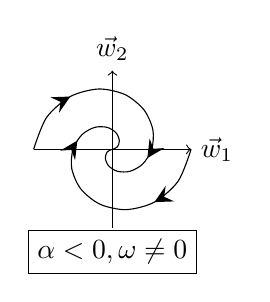
\begin{tikzpicture}
    \draw[->] (-1,0) -- (1,0) node[right] {$\vec{w}_1$};
     \draw[->] (0,-1) -- (0,1) node[above] {$\vec{w}_2$};
	\draw[smooth, samples=15, domain=1:0] plot({\x*cos(360*\x)}, {\x*sin(360*\x)}) [arrow inside={end=stealth,opt={scale=2}}{0.25, 0.75}];
	\draw[smooth, samples=15, domain=1:0] plot({-\x*cos(360*\x)}, {-\x*sin(360*\x)}) [arrow inside={end=stealth,opt={scale=2}}{0.25, 0.75}];
     \node[draw] at (0, -1.3) {$\alpha<0, \omega\neq0$};
	\end{tikzpicture}
	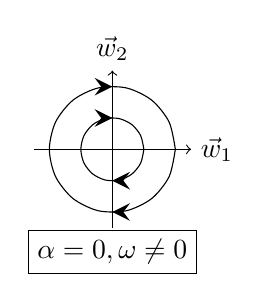
\begin{tikzpicture}
    \draw[->] (-1,0) -- (1,0) node[right] {$\vec{w}_1$};
     \draw[->] (0,-1) -- (0,1) node[above] {$\vec{w}_2$};
     \draw[smooth, samples=15, domain=1:0] plot({0.8*cos(360*\x)}, {0.8*sin(360*\x)}) [arrow inside={end=stealth,opt={scale=2}}{0.25, 0.75}];
	\draw[smooth, samples=15, domain=1:0] plot({0.4*cos(360*\x)}, {0.4*sin(360*\x)}) [arrow inside={end=stealth,opt={scale=2}}{0.25, 0.75}];
     \node[draw] at (0, -1.3) {$\alpha=0, \omega\neq0$};
	\end{tikzpicture}
\end{center}

\subsection{Limit Cycles}
Can also have limit cycles, where instead of a fixed point, there might be a fixed trajectory that the system is attracted to, eg the circle with constant $r=R$.
We would expand around this radius and evaluate the system there:
\begin{center}
	\begin{tikzpicture}
    \draw[->] (-1,0) -- (1,0) node[right] {$\vec{w}_1$};
     \draw[->] (0,-1) -- (0,1) node[above] {$\vec{w}_2$};
	\draw[smooth, samples=15, domain=0:0.8] plot({\x*cos(360*\x)}, {\x*sin(360*\x)}) [arrow inside={end=stealth,opt={scale=2}}{0.25, 0.75}];
	\draw[smooth, samples=15, domain=0:0.8] plot({-\x*cos(360*\x)}, {-\x*sin(360*\x)}) [arrow inside={end=stealth,opt={scale=2}}{0.25, 0.75}];
     \draw[smooth, samples=15, domain=0:1] plot({0.8*cos(360*\x)}, {0.8*sin(360*\x)}) [arrow inside={end=stealth,opt={scale=2}}{0.01, 0.5}];
	\end{tikzpicture}
\end{center}
\subsection{Hamiltonian Behaviours}
For Hamiltonian systems, we have $\lambda_\pm=\pm\sqrt{-|\mathbf{A}|}$, and so there are only \textbf{elliptic} fixed points for $|\mathbf{A}|>0$ and \textbf{hyperbolic} fixed points for $|\mathbf{A}|<0$.

\section{Poisson Brackets}
The poisson bracket of two functions $f$ and $g$ is defined in a coordinate system with positions and momenta $\vec q, \vec p$ as:
\begin{equation}	
	\left\{f, g\right\}_{p, q} = \left(\frac{\partial f}{\partial q^i} \frac{\partial g}{\partial p_i}- \frac{\partial f}{\partial p_i} \frac{\partial g}{\partial q^i}\right)
\end{equation}

We have the equation of motion of an observable $A(\vec q, \vec p, t)$:
\begin{equation}
	\frac{d A}{dt} = \left\{A, H\right\} + \frac{\partial A}{\partial t}
\end{equation}
Hamilton's equations of motion can be written:
\begin{align}
	\dot {\vec q} &= \left\{\vec{q}, H\right\} & \dot {\vec p} &= \left\{\vec{p}, H\right\}
\end{align}
If A is a constant of the motion:
\begin{align}
	\frac{d A}{dt}&=0,&\mathrm{then,} &&\left\{A, H\right\} &=\frac{\partial A}{\partial t} 
\end{align}
If $u$ and $v$ are constants of motion, then $\left\{u, v\right\}$ is a constant of motion too.
\section{Canonical Transformations}
Canonical transformations are a transformation of the coordinates $\vec{q}, \vec{p}, H \rightarrow \vec{Q}(\vec{q}, \vec{p}, t), \vec{P}(\vec{q}, \vec{p}, t), K$ that satisfies:
\begin{align}
	\dot{\vec Q}&=\frac{\partial K}{\partial \dot{\vec{P}}} & \dot{\vec P}&=-\frac{\partial K}{\partial \dot{\vec Q}}
\end{align}
Using the fact that the Euler-Lagrange equations are invariant under a total time derivative added to the Lagrangian, we find a generating function:
\begin{equation}
	\vec{p}\cdot\dot{\vec q}-H-(\vec{P}\cdot\dot{\vec Q}-K) = \frac{dF_1(\vec{q}, \vec{Q}, t)}{dt}
\label{eq:hamiltonian_kamiltonian}
\end{equation}
We can multiply equation \ref{eq:hamiltonian_kamiltonian} by $dt$ and look at the differential form of $F_1$ to see how to get $\vec{p}, \vec{P}$ from it:
\begin{align}
	dF_1 &= \vec{p}\cdot d\vec{q} - \vec{P}\cdot d\vec{Q} -(H-K)dt \\
	dF_1 &= \frac{\partial F_1}{\partial \vec{q}}\cdot d\vec{q} + \frac{\partial F_1}{\partial \vec{Q}}\cdot d\vec{Q} + \frac{\partial F_1}{\partial t}dt
\end{align}
Equating the coefficients:
\begin{align}
	\vec{p} &= \frac{\partial F_1}{\partial \vec{q}} & 
	\vec{P} &= -\frac{\partial F_1}{\partial \vec{Q}} &
	K &= H + \frac{\partial F_1}{\partial t}
\end{align}

If we have two sets of coordinates: $\vec\eta = (\vec q, \vec p)$ and $\vec\zeta = (\vec Q, \vec P)$, then the transformation between them is canonical if and only if:
\begin{equation}
	\left\{\zeta^i, \zeta^j\right\}_{\vec \eta} = 
	\begin{pmatrix}
		\mathbf{I} & \mathbf{0} \\
		\mathbf{0} & -\mathbf{I} 
	\end{pmatrix} = J^{ij}
\end{equation}

Where the $\mathbf{I}$ are block identity matrices.

We can use generating functions of different combinations of $q, p, Q, P$. These are all related by a Legendre transform:

\begin{align}
	F_2(\vec{q}, \vec{P}) &= F_1(\vec{q},\vec{Q})+\vec{Q}\cdot\vec{P} \\
	F_3(\vec{p}, \vec{Q}) &= F_1(\vec{q},\vec{Q})-\vec{q}\cdot \vec{p} \\
	F_4(\vec{p}, \vec{P}) &= F_1(\vec{q},\vec{Q})-\vec{q}\cdot\vec{p}+\vec{Q}\cdot\vec{P}
\end{align}
Under these generating functions, the equations for the other coordinates are:

\begin{align}
	F_1(\vec{q}, \vec{Q}): &&
	\vec{p} &= \frac{\partial F_1}{\partial \vec{q}} & 
	\vec{P} &= -\frac{\partial F_1}{\partial \vec{Q}} & \\
	F_2(\vec{q}, \vec{P}): &&
	\vec{p} &= \frac{\partial F_2}{\partial \vec{q}} & 
	\vec{Q} &= \frac{\partial F_2}{\partial \vec{P}} & \\
	F_3(\vec{p}, \vec{Q}): &&
	\vec{q} &= -\frac{\partial F_3}{\partial \vec{p}} & 
	\vec{P} &= -\frac{\partial F_3}{\partial \vec{Q}} & \\
	F_4(\vec{p}, \vec{P}): &&
	\vec{q} &= -\frac{\partial F_4}{\partial \vec{p}} & 
	\vec{Q} &= \frac{\partial F_4}{\partial \vec{P}} &
\end{align}

Under transformations with generating functions of the form $F_1=\vec{q}\cdot\vec{Q}$ and $F_4=\vec{p}\cdot\vec{P}$, we can perform an exchange transformation, where the old coordinates become the new moment and vice-versa. With generating functions of the form $F_2=\vec{q}\cdot\vec{P}$ and $F_3=-\vec{p}\cdot\vec{Q}$, we get an identity transformation.
\subsection{Infinitesimal Canonical Transformations}
Consider canonical transformations close to the indentity:
\begin{equation}
	F_2(\vec{q}, \vec{P}, t) = \vec{q}\cdot\vec{P} + \epsilon G(\vec{q}, \vec{P}, t)
\end{equation}
$G(\vec{q}, \vec{P}, t)$ is the generator of the infinitesimal canonical transform.
Considering the changes in coordinates and momenta under this transformation, we have:
\begin{align}
	\delta \vec{q} &= \vec{Q}-\vec{q} &= \epsilon \frac{\partial G(\vec{q},\vec{P},t)}{\partial \vec{P}} &=\epsilon \frac{\partial G(\vec{q},\vec{p},t)}{\partial \vec{p}} + O(\epsilon^2) \\
	\delta \vec{p} &= \vec{P}-\vec{p} &= -\epsilon \frac{\partial G(\vec{q},\vec{P},t)}{\partial \vec{q}}  &= -\epsilon \frac{\partial G(\vec{q},\vec{p},t)}{\partial \vec{q}} + O(\epsilon^2)
\end{align}
If some infinitesimal generator leaves the functional form of the Hamiltonian the same, then $H(\vec{Q}, \vec{P}, t) - H(\vec{q}, \vec{p}, t) = \epsilon\frac{\partial G}{\partial t}=-\epsilon\left\{G, H\right\}$, and the infinitesimal generator of the transformation is a constant of motion:
\begin{equation}
	\frac{dG}{dt} = \left\{G, H\right\} + \frac{\partial G}{\partial t} = 0
\end{equation}
We can iterate the poisson bracket of a variable with an infinitesimal canonical transformation to build up finite motions. Let $\hat Gu=\{G, u\}$, then we can take derivatives of $u$ with:
\begin{equation}
	\frac{du}{d\alpha} = -\hat Gu
\end{equation}
And can build up the taylor expansion of $u(\alpha)$:
\begin{equation}
	u(\alpha) = \sum_{n=0}^{\infty}\frac{(-\alpha)^n}{n!}\hat Gu(\alpha)|_{\alpha=0}= e^{-\alpha\hat G} u(\alpha)|_{\alpha=0}
\end{equation}

\section{Hamilton-Jacobi Theory}
Find a canonical transformation, $S(\vec{q}, \vec \alpha)$ that takes the coordinates $(\vec q, \vec p)$ to constant coordinates $(\vec \beta, \vec \alpha)$. We take the transformed Hamiltonian, $K(\vec \beta, \vec \alpha)=0$ to give the Hamilton-Jacobi equation:
\begin{equation}
	H(\vec q, \frac{\partial S}{\partial \vec{q}}, t) + \frac{\partial S}{\partial t} = 0
\end{equation}
For systems of constant energy with separable coordinates, we can look for solutions of the form:
\begin{equation}
	S(\vec q, \vec \alpha, t) = \sum_i W_i(q_i, \vec \alpha) - Et
\end{equation}

Where each $W_i(q_i, \vec \alpha)$ is a function of a coordinate and the transformed momenta.

\subsection{Constants of Motion}
Some function of coordinates $I(q, p)$ is a constant of motion if and only if $\left\{I, H\right\}=0$

If a set of constants of motion, $\mathcal{C}=\{I_i(q, p)\}$, all mutually commute ($\{I_i, I_j\} = 0,$ $\forall I_i, I_j \in \mathcal{C}$), then they are said to be in \textbf{involution} 
\subsection{Liouville's Theorem on Integrability}
If the phase space of some Hamiltonian with $f$ degrees of freedom is bounded, and there are $f$ constants of motion $\alpha_i$ in involution, then the motion in the new coordinates $\beta^i$ has constant velocity $\dot\beta^i=\frac{\partial H(\vec\alpha)}{\partial \alpha_i}=\omega^i$, and the system evolves on $f$-dimensional tori in the new coordinates.
\subsection{Action-Angle Coordinates}
Can define an action and angle variable $J_i, \theta_i$ for each of the coordinates $q_i$ of a time-independent Hamiltonian:
\begin{equation}
	J_i = \frac{1}{2\pi}\oint_{\mathrm{cycle}}p_idq_i
\end{equation}
Since the original Hamiltonian was time-independent, the new Hamiltonian has the same numerical value, with the new coordinates $H(\vec \theta, \vec J)$. 
Since $\vec J$ is constant then the new Hamiltonian is a function of $\vec J$ only:
\begin{equation}
	\frac{d J_i}{dt} = 0 = \frac{\partial H}{\partial \theta_i}
\end{equation}
And the frequencies of the angles are:
\begin{equation}
	\frac{d\theta^i}{dt} = \omega^i = \frac{\partial H}{\partial J_i}
\end{equation}
Over one cycle, the angle changes by $2\pi$:
\begin{equation}
	\Delta \theta^i = \oint \frac{\partial \theta^i}{\partial q^j}dq^j = \oint\frac{\partial W}{\partial q^j\partial J_i}dq^j=\frac{\partial}{\partial J_i}\oint p^jdq^j=2\pi
\end{equation}

\section{Canonical Perturbation Theory}
Look at perturbations to the Hamiltonian of the form $H=H_0+\epsilon H_1$. 
We first find solutions to the unperturbed Hamiltonian $H_0$, and the transformed variables $\vec \alpha_0, \vec \beta_0$. 
We can then find the progressively higher order corrections with the recursive equations:

\begin{align}
	\dot{\vec\beta}_n &=\frac{\partial H_1(\vec \beta_{n-1}, \vec \alpha_{n-1}, t)}{\vec \alpha_{n-1}} \\
	\dot{\vec\alpha}_n &=-\frac{\partial H_1(\vec \beta_{n-1}, \vec \alpha_{n-1}, t)}{\vec \beta_{n-1}}
\end{align}
Where the $(n-1^{th})$ term contains all terms of lower order.


\end{document}

\end{verbatim}

\rule{0.3\linewidth}{0.25pt}
\scriptsize


\end{multicols}
\end{document}
